\documentclass{article}
\usepackage{amsmath}
\usepackage{graphicx}
\usepackage{listings}
\usepackage[usenames,dvipsnames]{color} % more flexible names for syntax highlighting colors
\usepackage{listings}

\lstset{
basicstyle=\ttfamily, 
columns=fullflexible, % make sure to use fixed-width font, CM typewriter is NOT fixed width
stepnumber=1,              
numbersep=10pt, 
tabsize=4,
lineskip=-1.5pt,
extendedchars=true,
breaklines=true,        
keywordstyle=\color{Blue}\bfseries,
commentstyle=\sffamily\color{OliveGreen},
stringstyle=\color{Maroon},
showstringspaces=true,
upquote=false,
}

\lstdefinelanguage{julia}
{
  keywordsprefix=\@,
  morekeywords={
    exit,whos,edit,load,is,isa,isequal,typeof,tuple,ntuple,uid,hash,finalizer,convert,promote,
    subtype,typemin,typemax,realmin,realmax,sizeof,eps,promote_type,method_exists,applicable,
    invoke,dlopen,dlsym,system,error,throw,assert,new,Inf,Nan,pi,im,begin,while,for,in,return,
    break,continue,macro,quote,let,if,elseif,else,try,catch,end,bitstype,ccall,do,using,module,
    import,export,importall,baremodule,immutable,local,global,const,Bool,Int,Int8,Int16,Int32,
    Int64,Uint,Uint8,Uint16,Uint32,Uint64,Float32,Float64,Complex64,Complex128,Any,Nothing,None,
    function,type,typealias,abstract
  },
  sensitive=true,
  morecomment=[s]{\#=}{=\#},
  morestring=[b]',
  morestring=[b]" 
}
\title{Formulas}
\author{Juan Camilo Guevara Hernández}
\begin{document}
\maketitle
This document will talk about the physical analysis used to control two motors in a polar coordinate system. Each motor generates motion: one for the radius, and the other one for the angle. \\
The main objective is to determine two independent functions that calculate the time required based on $\Delta \theta$ and $\Delta r$.
This analysis assumes: Constant angular velocity in both motors, identical radius on both axis of the belt, perfect transmission between gearbox, perfect transmission between the belt and the pulleys.\\
\newpage
\section{Inputs}
\begin{itemize}
  \item Angular Motor: The motor responsible for changing the angle.
  \item Radial Motor: The motor that adjusts the radius of the system.
  \item Zp : Number of teeth on the pinion.  
  \item Zn : Number of teeth on the gear.  
  \item R : Radius of the axis
  \item $\omega_1$ : Angular velocity of the angular motor.
  \item $\omega_2$ : Angular velocity of the radial motor.
  \item $\omega_g$ : Angular velocity of the gear.
\end{itemize}
\begin{figure}[htbp]
  \centering
  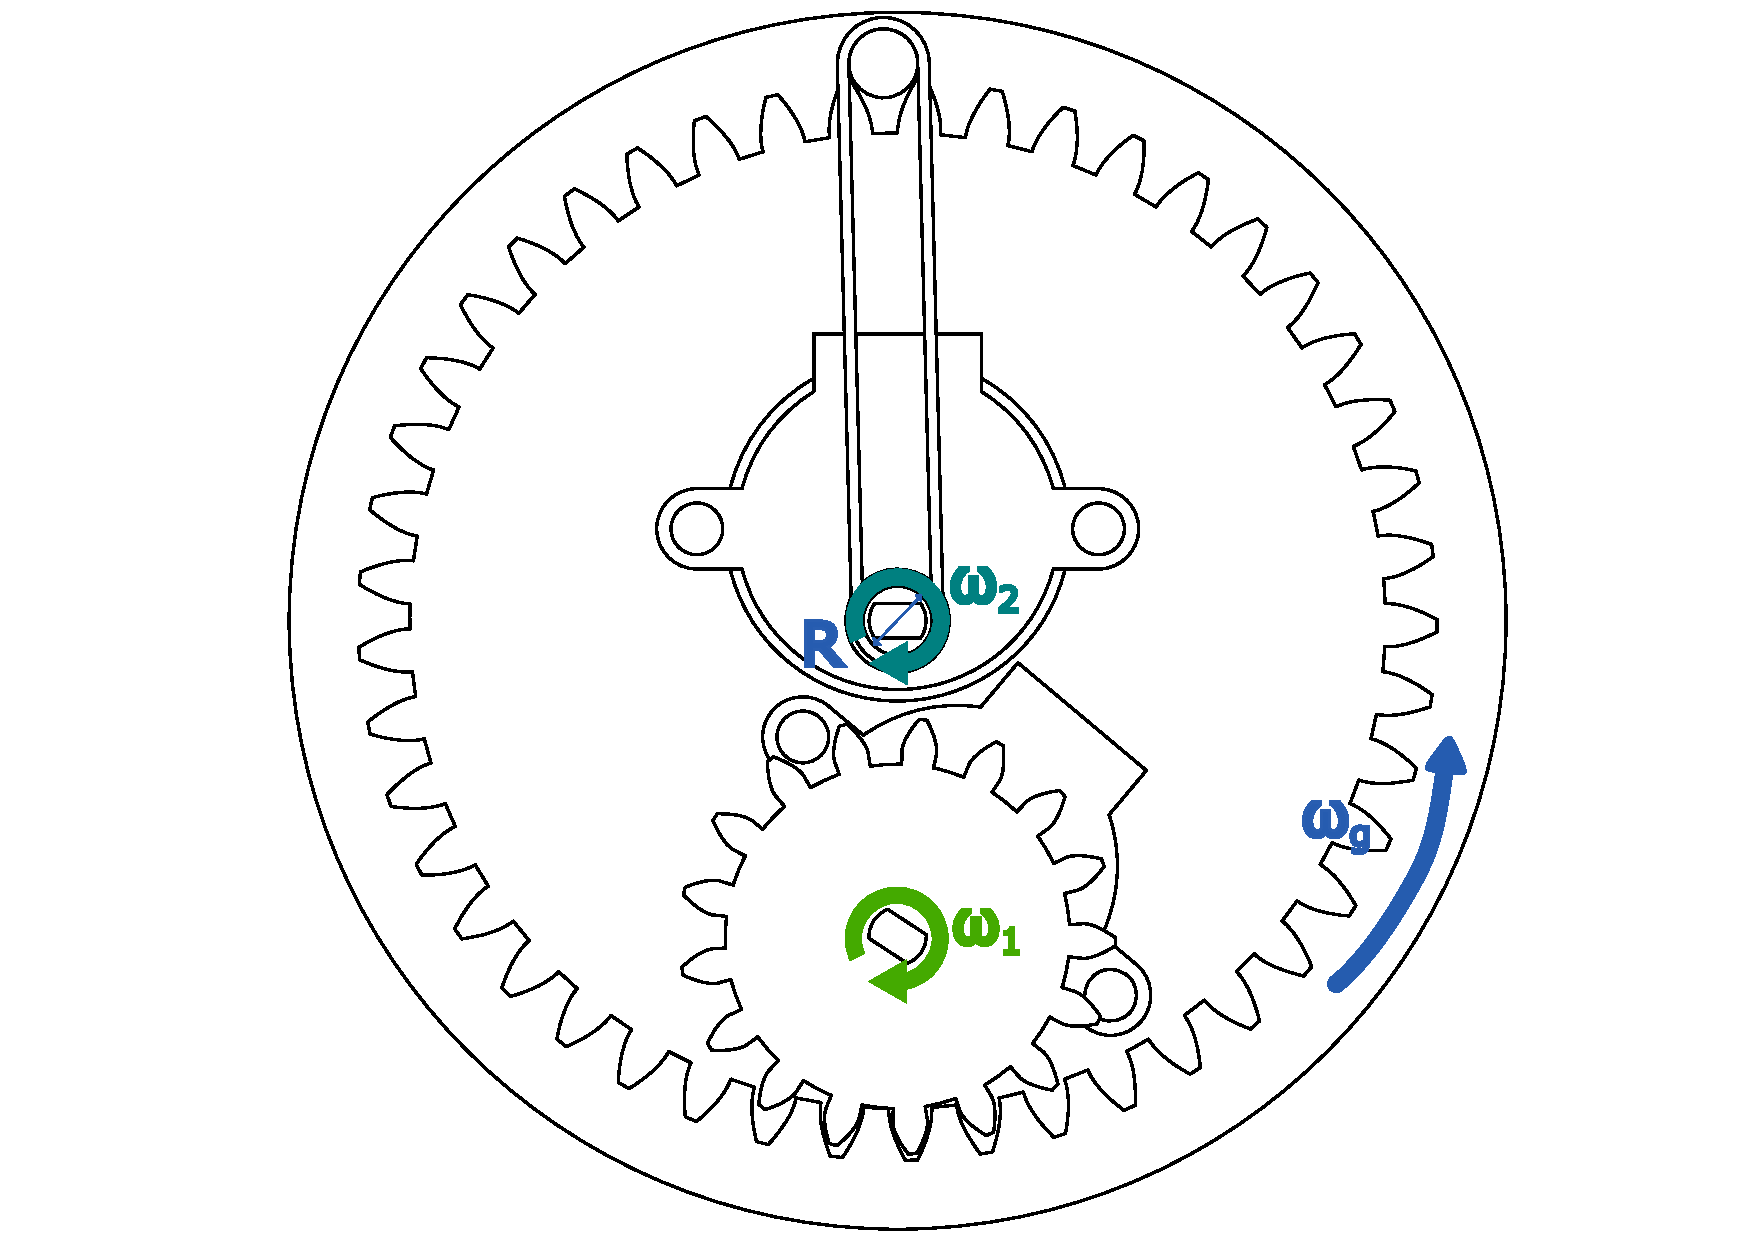
\includegraphics[scale=0.3]{./graph1.pdf}
\end{figure}
\section{Angular Motor}
To calculate the time the motor needs to be powered on, we will use the angular velocity of the gear as follows:
\begin{equation}
  \omega_g = \Delta\theta/t
\end{equation}
Now the $\omega_g$ is equal to the ration of the gear teeth as a reduction gearbox, multiplied by $\omega_1$. By substituting this into equation (1) and solving for $t$, we get:
\begin{equation}
  \begin{split}
    \frac{\Delta\theta}{t} &= (zp/zn) \cdot \omega_1\\
     t &= \frac{zn}{zp \cdot \omega_1}\Delta\theta 
  \end{split}
\end{equation}
\section{Radial Motor}
To calculate the time the motor needs to remain powered on to move a point $r_i$ along a belt to a target point $r_f$ we need the radius of the axis circle, $R$. \\
Using the formula $\Delta r = 2\pi R \cdot \textit{revolutions}$ and the relationship between a revolution and the angular velocity of the radial motor ($\omega_2$) we can state the following:
\begin{equation}
  \begin{split}
    \Delta r = 2R\pi \cdot \textit{revolutions} \\
    \textit{revolutions} = (\omega_2 \cdot t)/2\pi
  \end{split}
\end{equation}
Thus, solving for $t$, we obtain:
\begin{equation}
  \begin{split}
    \Delta r &= 2R\pi \cdot \frac{\omega_2 \cdot t}{2\pi} \\
    \Delta r &= R \cdot \omega_2 \cdot t \\
    t &= \frac{\Delta r}{\omega_2 \cdot R}
  \end{split}
\end{equation}
\section{Code implementation with Julia}
\lstinputlisting[language=Julia, firstline=4, lastline=40]{../src/Simulation.jl}
\begin{lstlisting}
  (3.0, 13.23529411764706)
\end{lstlisting}
\end{document}
